\ifdefined\pdfoutput\else\newcount\pdfoutput\fi % lets XeLaTeX read the next line
\pdfoutput=1 % arXiv: compile with pdfLaTeX (keep within the first five lines)
\ifdefined\XeTeXversion\pdfoutput=0\fi % XeTeX and Tectonic: restore the default
\documentclass[11pt]{amsart}

% ---------------------------------------------------------------------------
% Engine-neutral preamble: compiles under pdfLaTeX (arXiv default) and XeTeX.
% The source is kept pure ASCII.
% ---------------------------------------------------------------------------
\usepackage{iftex}
\ifPDFTeX
  \usepackage[utf8]{inputenc}
  \usepackage[T1]{fontenc}
\fi
\usepackage{lmodern}
\usepackage{amsmath,amssymb,amsthm,mathtools}
\usepackage[margin=1.15in]{geometry}
\usepackage{booktabs}
\usepackage{array}
\usepackage{enumitem}
\usepackage{xcolor}
\usepackage{listings}
\usepackage{url}
\usepackage{tikz}
\usetikzlibrary{positioning,arrows.meta}
\usepackage{tikz-cd}
\usepackage[colorlinks=true,linkcolor=blue!50!black,citecolor=green!40!black,urlcolor=blue!60!black]{hyperref}
\hypersetup{
  pdftitle={A proof of the Applegate-Lagarias Conjecture A and the 3x+1 growth exponent conjecture},
  pdfauthor={Naoufal El Jaouhari},
  pdfsubject={Positive density of 3x+1 (Collatz) predecessors, proved and formally verified in Lean 4},
  pdfkeywords={3x+1 problem, Collatz problem, 3x-1 problem, inverse iterates, predecessor density,
    Applegate-Lagarias conjectures, growth exponent, Lean 4, formal verification}
}

% ---------------------------------------------------------------------------
% Lean listings (Unicode is written as escaped math so the file stays ASCII).
% ---------------------------------------------------------------------------
\lstdefinelanguage{lean}{
  morekeywords={theorem,lemma,def,example,noncomputable,fun,if,then,else,by,exact},
  sensitive=true,
  morecomment=[l]{--},
  morecomment=[s]{/-}{-/}
}
\lstset{
  language=lean,
  basicstyle=\ttfamily\footnotesize,
  keywordstyle=\bfseries,
  commentstyle=\itshape\color{black!60},
  columns=fullflexible,
  keepspaces=true,
  frame=single,
  framerule=0.3pt,
  xleftmargin=4pt,
  xrightmargin=4pt,
  aboveskip=8pt,
  belowskip=8pt,
  escapeinside={(*}{*)}
}

% ---------------------------------------------------------------------------
\newtheorem{theorem}{Theorem}[section]
\newtheorem{lemma}[theorem]{Lemma}
\newtheorem{proposition}[theorem]{Proposition}
\newtheorem{corollary}[theorem]{Corollary}
\newtheorem{conjecture}[theorem]{Conjecture}
\newtheorem*{theoremA}{Theorem A}
\newtheorem*{theoremB}{Theorem B}
\newtheorem*{theoremC}{Theorem C}
\theoremstyle{definition}
\newtheorem{definition}[theorem]{Definition}
\theoremstyle{remark}
\newtheorem{remark}[theorem]{Remark}

\newcommand{\Z}{\mathbb{Z}}
\newcommand{\N}{\mathbb{N}}
\newcommand{\R}{\mathbb{R}}
\newcommand{\Cp}{C_{+}}
\newcommand{\Cm}{C_{-}}
\newcommand{\Sp}{S_{+}}
\newcommand{\Sm}{S_{-}}
\newcommand{\reach}[1]{\mathrel{\rightsquigarrow_{#1}}}
\newcommand{\E}{\mathcal{E}}
% Keeps the x of the running head lowercase under amsart's uppercasing.
\DeclareRobustCommand*{\xvar}{x}
% Lean names: typewriter, breakable after dots and underscores.
\DeclareUrlCommand\lean{\urlstyle{tt}\Urlmuskip=0mu plus 1.5mu\relax}
\makeatletter
\g@addto@macro{\UrlBreaks}{\do\_\do\.}
\makeatother
\emergencystretch=2.5em
\raggedbottom

\begin{document}

\title[Conjecture~A and the $3\xvar+1$ growth exponent conjecture]%
{A proof of the Applegate--Lagarias Conjecture~A\\ and the $3x+1$ growth exponent conjecture}

\author{Naoufal El Jaouhari}
\address{Independent researcher}
\email{neljaouh@gmail.com}

\subjclass[2020]{Primary 11B83; Secondary 37P99, 11B37, 68V20}
\keywords{$3x+1$ problem, Collatz problem, $3x-1$ problem, inverse iterates, predecessor
density, Applegate--Lagarias conjectures, growth exponent, formal verification}

\date{September 2026}

\begin{abstract}
For an integer $a$ let $\pi_a(x)$ be the number of integers $n$ with $|n|\le x$ whose trajectory
under the $3x+1$ map $T$, given by $T(n)=n/2$ for even $n$ and $T(n)=(3n+1)/2$ for odd $n$,
contains~$a$. In 1995 Applegate and Lagarias conjectured that for every $a$ not divisible by~$3$
there is $c_a>0$ with $\pi_a(x)\ge c_a x$ for all $x\ge |a|$ (Conjecture~A). We prove this
conjecture. For positive targets the input is a recently released theorem, formally verified in
Lean: the predecessors of each positive target prime to~$3$ under the ordinary map
$n\mapsto n/2,\,3n+1$ have positive lower density. Negative targets require new mathematics. Negation conjugates the
$3x+1$ dynamics on the negative integers to the $3x-1$ dynamics on the positive integers, and we
prove the corresponding density theorem for $3x-1$. Its proof follows the architecture of the proof of that theorem. The
sign change reverses one basic inequality, which costs a multiplicative factor at every generation
of the inverse construction. We show that the product of these factors stays uniformly bounded.
Ordinary and accelerated predecessor sets can differ only at targets $a\equiv 4\pmod 6$, where
$T(2a)=a$ transfers the bound, and the target's membership in its own predecessor set gives the
bound for every $x\ge|a|$. As a corollary, $\log\pi_a(x)/\log x\to1$, which proves the $3x+1$
growth exponent conjecture. The complete argument, including the imported theorem, is formalized in
Lean~4 with Mathlib and has been replayed independently by the Lean kernel.
\end{abstract}

\maketitle

% ===========================================================================
\section{Introduction}\label{sec:intro}
% ===========================================================================

\subsection{Inverse iterates of the \texorpdfstring{$3x+1$}{3x+1} map}
Let $T\colon\Z\to\Z$ be the $3x+1$ map in the form used by Applegate and Lagarias
\cite[(1.1)]{AL95a},
\[
  T(n)=\begin{cases} (3n+1)/2, & n\text{ odd},\\ n/2, & n\text{ even}.\end{cases}
\]
The $3x+1$ conjecture asserts that every positive integer eventually reaches $1$. A way to measure
what is known is to fix a target $a$ and count the integers whose trajectories pass through it. Following \cite[(1.2)]{AL95a}, set
\begin{equation}\label{eq:pi}
  \pi_a(x)=\#\{\,n\in\Z:\ |n|\le x\ \text{and}\ T^{(k)}(n)=a\ \text{for some}\ k\ge0\,\}.
\end{equation}
If $3\mid a$, the only predecessors of $a$ are the numbers $2^ja$, so $\pi_a(x)$ grows
logarithmically. For $a\not\equiv0\pmod3$ the count grows at least like a power of~$x$: the
exponent $0.65$ was obtained in \cite[Theorem~1.2]{AL95a}, where the earlier bounds are surveyed
\cite[\S1]{AL95a}, and the exponent $0.84$ is recorded in \cite[Theorem~2.5]{KontorovichLagarias10}.
Applegate and Lagarias conjectured that the growth is in fact linear.

\begin{conjecture}[Applegate--Lagarias {\cite[Conjecture~A]{AL95a}}]\label{conj:A}
For each $a\not\equiv0\pmod3$ there is a positive constant $c_a$ such that $\pi_a(x)\ge c_a x$ for
all $x\ge|a|$.
\end{conjecture}

Kontorovich and Lagarias \cite[Definition~2.11]{KontorovichLagarias10} define the upper and lower
growth exponents
\[
  \eta_3^{+}(a)=\limsup_{x\to\infty}\frac{\log\pi_a(x)}{\log x},\qquad
  \eta_3^{-}(a)=\liminf_{x\to\infty}\frac{\log\pi_a(x)}{\log x},
\]
and record the following conjecture, which they attribute to Applegate and Lagarias and note is
weaker than Conjecture~\ref{conj:A}.

\begin{conjecture}[$3x+1$ growth exponent conjecture {\cite[Conjecture~2.1]{KontorovichLagarias10}}]
\label{conj:growth}
For every integer $a\not\equiv0\pmod3$ the growth exponent exists and equals one:
$\eta_3^{+}(a)=\eta_3^{-}(a)=1$.
\end{conjecture}

Both conjectures are predicted by stochastic models of the inverse iteration
\cite{KontorovichLagarias10}.

\subsection{Main results}

\begin{theoremA}[Conjecture~A]
For every $a\in\Z$ with $3\nmid a$ there is $c_a>0$ such that $\pi_a(x)\ge c_a x$ for every real
$x\ge|a|$.
\end{theoremA}

\begin{theoremB}[Growth exponents]
For every $a\in\Z$ with $3\nmid a$,
\[
  \lim_{x\to\infty}\frac{\log\pi_a(x)}{\log x}=1 .
\]
In particular $\eta_3^{+}(a)=\eta_3^{-}(a)=1$, which proves Conjecture~\ref{conj:growth}.
\end{theoremB}

The negative targets of Theorem~A rest on a density theorem for the $3x-1$ map
$\Cm(m)=m/2$ for even $m$, $\Cm(m)=3m-1$ for odd $m$.

\begin{theoremC}[Predecessor density for $3x-1$]
For every integer $a\ge1$ with $3\nmid a$, the set $\{m\ge1:\ \Cm^{k}(m)=a\text{ for some }k\ge0\}$
has positive lower natural density.
\end{theoremC}

\subsection{From the positive-target theorem to Conjecture~A}
The positive-target input is the predecessor-density theorem of \cite{MazurM2}, stated as
Theorem~\ref{thm:input} in Section~\ref{sec:prelim}. It differs from Conjecture~A in four respects.

\begin{center}
\small
\begin{tabular}{@{}llll@{}}
\toprule
 & Theorem~\ref{thm:input} & Conjecture A & What is needed \\
\midrule
map & ordinary $\Cp$ & accelerated $T$ & elementary except at $a\equiv4\ (6)$; Section~\ref{sec:accel} \\
target & $a\ge1$ & $a\in\Z$ & \textbf{new theorem for $3x-1$}; Sections~\ref{sec:minus},~\ref{sec:neg} \\
starting points & $n\ge1$ & $n\in\Z$ & embedding, and negation for $a<0$ \\
cutoff & integer $X\ge X_a$ & every real $x\ge|a|$ & elementary; Section~\ref{sec:proofA} \\
\bottomrule
\end{tabular}
\end{center}

\noindent Three of the four gaps are closed by elementary arguments. The second is not. The
dynamics of $T$ on the negative integers is the $3x-1$ dynamics in disguise
(Lemma~\ref{lem:conj}), and no density theorem for $3x-1$ was available.

\subsection{Contributions and relation to prior work}
\begin{enumerate}[leftmargin=*,label=(\roman*)]
\item \emph{Theorem~C} (Section~\ref{sec:minus}). It is proved by running the argument of \cite{MazurM1,MazurM2} for the
  $3x-1$ map. We identify the four places where the sign of the $\pm1$ enters. Residue conditions
  transfer exactly under the negation $z\mapsto -z$ of $3$-adic residues
  (Lemma~\ref{lem:neg-correspondence}). The one inequality that reverses is the charge inequality
  $x_w\omega(w)\le R$ between a source, its weight and its root. It is repaired by a sharp charge
  bound (Lemma~\ref{lem:sharp-charge}) whose excess is summable along the scale recursion, so the
  accumulated loss is bounded by an absolute constant $\E<1+5\cdot10^{-50}$
  (Lemma~\ref{lem:product}).
\item \emph{The signed assembly} (Sections~\ref{sec:accel}--\ref{sec:proofA}). The conjugacy
  $\Cp(-m)=-\Cm(m)$ carries Theorem~C to negative targets. An ordinary-to-accelerated bridge
  handles the map, and a threshold argument gives the exact form of Conjecture~A. For positive
  targets the bridge is already noted in \cite[\S1.2]{MazurM2}: Theorem~\ref{thm:input}, applied
  to~$2a$, yields positive density for~$T$.
\item \emph{Theorem~B} (Section~\ref{sec:growth}), a short consequence of Theorem~A.
\end{enumerate}
Theorem~\ref{thm:input} is the only imported result. Its human-readable proof is in the
manuscripts \cite{MazurM1,MazurM2}, which have not been refereed. Section~\ref{subsec:input}
records their provenance and Section~\ref{sec:limits} discusses what it implies.

\subsection{The formal proof}
Theorems~A, B and~C, together with Theorem~\ref{thm:input} and every lemma used to derive them, are
formally proved in Lean~4 \cite{Lean4} with Mathlib \cite{Mathlib}. The development depends only
on Lean's three standard axioms, and the Lean kernel has independently replayed it. Both
conjectures are restated in Lean from first principles and discharged by the main theorems, which
checks that the formal statements are the published ones. Section~\ref{sec:verification} gives
the details.

\subsection{Organization}
Figure~\ref{fig:architecture} shows the structure of the proof. Section~\ref{sec:prelim} sets up
notation, states Theorem~\ref{thm:input} and describes the steps of its proof. Section~\ref{sec:minus} proves
Theorem~C. Sections~\ref{sec:accel} and~\ref{sec:neg} pass to the accelerated map and to negative
targets. Section~\ref{sec:proofA} proves Theorem~A and Section~\ref{sec:growth} proves Theorem~B.
Section~\ref{sec:verification} describes the formal verification, Section~\ref{sec:limits}
discusses the constants and the scope of the result, and Section~\ref{sec:further} lists further
questions.

\begin{figure}[t]
\centering
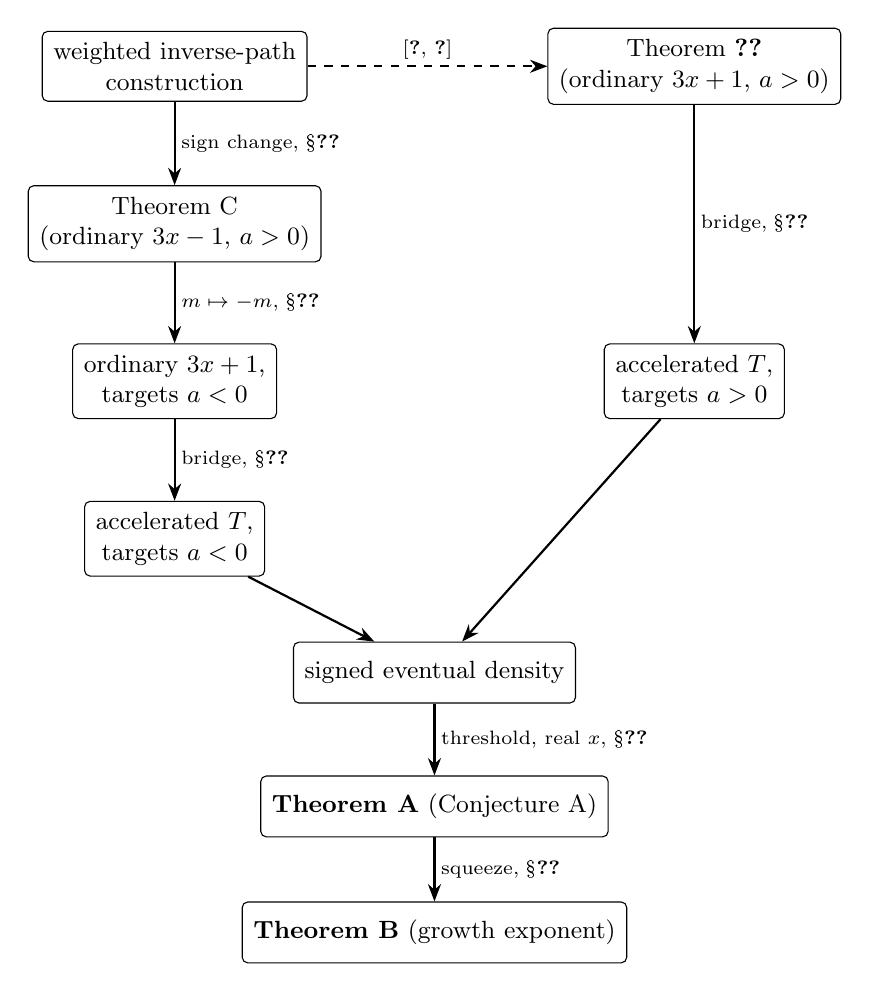
\begin{tikzpicture}[
  box/.style={draw,rounded corners=2pt,align=center,font=\small,inner sep=4pt,minimum height=2.2em},
  arr/.style={-{Stealth[length=2.2mm]},thick},
  lab/.style={font=\scriptsize,align=left,inner sep=2pt}]
\node[box] (mech) at (0,0) {weighted inverse-path\\construction};
\node[box] (M) at (6.6,0) {Theorem~\ref{thm:input}\\(ordinary $3x+1$, $a>0$)};
\node[box] (C) at (0,-2.0) {Theorem C\\(ordinary $3x-1$, $a>0$)};
\node[box] (neg) at (0,-4.0) {ordinary $3x+1$,\\ targets $a<0$};
\node[box] (accneg) at (0,-6.0) {accelerated $T$,\\ targets $a<0$};
\node[box] (accpos) at (6.6,-4.0) {accelerated $T$,\\ targets $a>0$};
\node[box] (ev) at (3.3,-7.7) {signed eventual density};
\node[box] (A) at (3.3,-9.4) {\textbf{Theorem A} (Conjecture A)};
\node[box] (B) at (3.3,-11.0) {\textbf{Theorem B} (growth exponent)};
\draw[arr] (mech) -- node[lab,right] {sign change, \S\ref{sec:minus}} (C);
\draw[arr,dashed] (mech) -- node[lab,above] {\cite{MazurM1,MazurM2}} (M);
\draw[arr] (C) -- node[lab,right] {$m\mapsto -m$, \S\ref{sec:neg}} (neg);
\draw[arr] (neg) -- node[lab,right] {bridge, \S\ref{sec:accel}} (accneg);
\draw[arr] (M) -- node[lab,right] {bridge, \S\ref{sec:accel}} (accpos);
\draw[arr] (accneg) -- (ev);
\draw[arr] (accpos) -- (ev);
\draw[arr] (ev) -- node[lab,right] {threshold, real $x$, \S\ref{sec:proofA}} (A);
\draw[arr] (A) -- node[lab,right] {squeeze, \S\ref{sec:growth}} (B);
\end{tikzpicture}
\caption{Structure of the proof. The dashed arrow is the imported theorem, proved in
\cite{MazurM1,MazurM2}. Theorem C reuses the construction behind Theorem~\ref{thm:input}, not
Theorem~\ref{thm:input} itself.}
\label{fig:architecture}
\end{figure}

% ===========================================================================
\section{Preliminaries and the input theorem}\label{sec:prelim}
% ===========================================================================

\subsection{Maps, reachability, density}
Besides $T$ we use the ordinary maps
\[
  \Cp(n)=\begin{cases} 3n+1, & n\text{ odd},\\ n/2, & n\text{ even},\end{cases}\qquad
  \Cm(n)=\begin{cases} 3n-1, & n\text{ odd},\\ n/2, & n\text{ even},\end{cases}
\]
with $\Cp$ defined on $\Z$ and $\Cm$ on the positive integers, which it preserves. For a map $f$
write $n\reach{f}a$ if $f^{k}(n)=a$ for some $k\ge0$; the case $k=0$ is allowed, so $a\reach{f}a$.
For a set $A$ of positive integers and $X\in\N$ let $A(X)=\#\{n\in A: n<X\}$. The set $A$ has
\emph{positive lower density} if there are $c>0$ and $X_0$ with $A(X)\ge cX$ for every integer
$X\ge X_0$. We write $G_k=\Z/3^k\Z$ and $\langle f\rangle_k=3^{-k}\sum_{z\in G_k}f(z)$ for
$f\colon G_k\to\R$.

\subsection{Syracuse maps and exact words}
For a positive odd integer $x$ put
\[
  \Sp(x)=\frac{3x+1}{2^{v_2(3x+1)}},\qquad \Sm(x)=\frac{3x-1}{2^{v_2(3x-1)}} .
\]
Both are maps of the positive odd integers to themselves. The ordinary orbit of an odd $x$ under
$C_\pm$ passes through $S_\pm(x)$. Hence $x\reach{S_\pm}R$ implies $x\reach{C_\pm}R$.

\begin{definition}\label{def:words}
Let $R$ be a positive odd integer. A finite sequence $w=(a_1,\dots,a_d)$ of positive integers is an
\emph{exact word for $S_\pm$ ending at $R$} if there is a positive odd integer $x_w$, the
\emph{source}, with $S_\pm^{d}(x_w)=R$ and $a_i=v_2\bigl(3S_\pm^{i-1}(x_w)\pm1\bigr)$ for
$1\le i\le d$. We write $d=d(w)$, $A(w)=a_1+\dots+a_d$, and define the \emph{weight} and the
\emph{offset}
\[
  \omega(w)=3^{d}\,2^{-A(w)},\qquad
  B_w=\sum_{i=1}^{d}3^{\,d-i}\,2^{\,a_1+\dots+a_{i-1}} .
\]
\end{definition}

The weight is the one used in \cite[(2.1)]{MazurM1} and \cite[(3.1)]{MazurM2}. The weight and the
offset depend only on the word, not on the sign. Iterating $3x\pm1=2^{a}S_\pm(x)$ along the orbit
gives, by induction on $d$,
\begin{equation}\label{eq:affine}
  3^{d}x_w\pm B_w=2^{A(w)}R,\qquad\text{equivalently}\qquad x_w\,\omega(w)=R\mp\frac{B_w}{2^{A(w)}} .
\end{equation}
For $3x+1$ this gives the \emph{charge inequality} of \cite[(3.2)]{MazurM2},
\begin{equation}\label{eq:charge-plus}
  x_w\,\omega(w)\le R\qquad(\text{sign }+).
\end{equation} For $3x-1$ the same identity gives $x_w\,\omega(w)\ge R$ instead.

\subsection{The input theorem}\label{subsec:input}

\begin{theorem}[Positive density of $3x+1$ predecessors {\cite[Theorem~1.1]{MazurM2}}]
\label{thm:input}
For every integer $a\ge1$ with $3\nmid a$, the set $P(a)=\{n\ge1:\ n\reach{\Cp}a\}$ has positive
lower density.
\end{theorem}

The statement allows even targets and assumes neither that $a$ reaches $1$ nor that $a$ is
nonperiodic. Its constants depend on $a$.

\emph{Provenance.} Theorem~\ref{thm:input} was released in September 2026 on the ProofAtlas
platform, as the manuscript \cite{MazurM2} with a Lean development built on the library of
\cite{MazurM1}. The manuscripts state that the research was directed by their author and that
generative AI (OpenAI models used through the ProofAtlas harness) contributed substantially to the
mathematical exploration, the proof development, the formalization and the exposition. Neither
manuscript reports human peer review. We therefore do not take the correctness of
Theorem~\ref{thm:input} on the authority of its exposition. It rests on the formal proof, which we
replayed independently in a fresh kernel environment (Section~\ref{sec:verification}). The manuscripts
serve here as the human-readable description of the proof's structure.

\subsection{The structure of the proof of Theorem~\ref{thm:input}}\label{subsec:anatomy}
The proof in \cite{MazurM2} combines five steps. Steps (P1), (P3), (P4) and (P5) are proved in
\cite{MazurM2}. Step (P2) is assembled there from the estimates of \cite{MazurM1}, in its Appendix~A.
\begin{enumerate}[leftmargin=*,label=(P\arabic*)]
\item \emph{Seeds} \cite[\S2]{MazurM2}. For every modulus $3^q$, every residue $y$ and every $L$
  there is a positive odd $R>L$ with $R\equiv y\pmod{3^q}$, $R\reach{\Cp}a$, and no positive
  return, that is, $\Sp^{t}(R)\ne R$ for all $t\ge1$. The seeds come from the explicit family
  $R_k=((3r_0+1)4^k-1)/3$, which runs through all residues modulo $3^q$. No return for large $R$
  comes from a lemma valid for every map $f\colon\N\to\N$ \cite[Lemma~2.1]{MazurM2}.
\item \emph{A residue-weighted mass} \cite[Proposition~3.1 and Appendix~A]{MazurM2},
  \cite[\S\S2--6, 8]{MazurM1}. Starting from a seed, inverse histories are built generation by
  generation. At generation $j$ one appends an exact word that first crosses a prescribed linear
  barrier at scale $b_j$, with bounded overshoot, where $b_0=2^{80}$ and $b_{j+1}=b_j+\lfloor
  b_j/100\rfloor$. The endpoint of each history becomes a root for the next generation. Each
  history is paired with a reference density $\rho_k\colon G_k\to[0,\infty)$ evaluated at its
  current endpoint. This density comes from the $3$-adic random walk
  $Y_{k+1}=2^{-E_{k+1}}(3Y_k+1)$ with independent geometric $E_j$, so it has mean $2/3$ and
  vanishes on nonunits. A finite-distribution mixing estimate gives
  $\langle|\rho_k-\rho_m\circ\pi_{k,m}|\rangle_k\le C/m^2$
  with an explicit constant~$C$ \cite[Lemma~8.1]{MazurM1}. Averaging over residues selects a unit
  residue $y$ at which the initial mark is at least $255/256$. Summable variation estimates show
  that the mark stays at least $175/256>2/3$ at every late generation, uniformly in the external
  scale $X$.
  Terminal sources lie in $[X,32X)$.
\item \emph{Distinct sources} \cite[Lemma~4.1]{MazurM2}. If the seed has no positive return, two
  words ending at it with the same source must have the same length, and hence coincide. So
  $w\mapsto x_w$ is injective, and by \eqref{eq:charge-plus} the words contribute weight at most
  $R/X$ to each distinct source in $[X,\infty)$.
\item \emph{Removing the residue weight} \cite[\S4.2]{MazurM2}. A residue-class count and the
  mixing estimate at a fixed coarse modulus $3^m$, with $m=132RC+1$, turn the weighted mass into a
  lower bound $U\ge\eta=3/(8\cdot3^m)$ for the total weight of the selected words.
\item \emph{Counting} \cite[\S4.3]{MazurM2}. Steps (P3) and (P4) give at least $XU/R$ distinct
  predecessors in $[X,32X)$. This yields Theorem~\ref{thm:input} with
  $c_a=3/(256\,R\,3^m)$ and $X_a=32(H+1)$ for a height $H$ depending on $R$.
\end{enumerate}

The sign of the $\pm1$ enters this proof at four points. We use this list in
Section~\ref{sec:minus}.
\begin{enumerate}[leftmargin=*,label=(S\arabic*)]
\item the Syracuse map itself, hence which words are exact and what the seeds are (P1);
\item the affine identity \eqref{eq:affine}, through the congruence that makes a word exact and
  through the residue maps and transfer operators of \cite[\S2]{MazurM1} (P2);
\item the charge inequality \eqref{eq:charge-plus} and the block-size bounds derived from it,
  \cite[(3.5)]{MazurM1}, which enter the histogram and variation estimates (P2), the source
  window (P2) and the count (P3), (P5);
\item the reduction of a terminal valuation by even amounts, which acts on sources by the affine
  map $\Psi_j(x)=4^jx+(4^j-1)/3$ (P2), (P4).
\end{enumerate}
The rest is independent of the sign. This includes the combinatorics of words (first crossings,
overshoot and length restrictions), their geometric probabilities, the mixing estimate, the
summable variation majorants, the scale-coverage argument and the non-return lemma.

% ===========================================================================
\section{Positive predecessor density for the \texorpdfstring{$3x-1$}{3x-1} map}\label{sec:minus}
% ===========================================================================

We prove Theorem~C by running the proof of Theorem~\ref{thm:input} for $\Sm$ and $\Cm$. We do not reprove the
sign-independent estimates of \cite{MazurM1,MazurM2}; we prove the statements that replace the
four sign-sensitive points (S1)--(S4) and track the constants they change.

\subsection{Exact words for \texorpdfstring{$3x-1$}{3x-1}}
For $\Sm$ the identity \eqref{eq:affine} reads $3^{d}x_w=2^{A(w)}R+B_w$. Unlike the $3x+1$ case,
no condition is needed to keep the source positive.

\begin{lemma}[Decoding]\label{lem:decode}
Let $R$ be a positive odd integer and $w=(a_1,\dots,a_d)$ a word of positive integers. If
$3^{d}\mid 2^{A(w)}R+B_w$, then $w$ is an exact word for $\Sm$ ending at $R$, with source
$x_w=(2^{A(w)}R+B_w)/3^{d}$.
\end{lemma}

\begin{proof}
Define $y_d=R$ and $y_{i-1}=(2^{a_i}y_i+1)/3$. These are rationals whose denominators are powers
of $3$, and $y_0=(2^{A(w)}R+B_w)/3^{d}$ by the computation behind \eqref{eq:affine}, so $y_0$ is an
integer by hypothesis. If $y_i$ were not an integer, then $v_3(y_i)<0$ and
$v_3(y_{i-1})=v_3(y_i)-1<0$, since $v_3(2^{a_i}y_i+1)=v_3(y_i)$. Inductively $y_0$ would not be
an integer. Hence every $y_i$ is an integer, and by downward induction every $y_i$ is positive.
Since $2^{a_i}y_i+1$ is odd, so is $y_{i-1}$. Finally $3y_{i-1}-1=2^{a_i}y_i$ with $y_i$ odd, so
$v_2(3y_{i-1}-1)=a_i$ and $\Sm(y_{i-1})=y_i$.
\end{proof}

\subsection{The negation correspondence}
A word is exact for $\Sm$ at $R$ if and only if $2^{A(w)}R\equiv-B_w\pmod{3^{d}}$. A word is exact
for $\Sp$ at $R'$ only if $2^{A(w)}R'\equiv B_w\pmod{3^{d}}$. So the $3x-1$ condition at $R$ is the
$3x+1$ condition at the residue $-R$. The next lemma makes this precise for every residue
statement, not only for exactness.

\begin{lemma}[Negation correspondence]\label{lem:neg-correspondence}
Let $w$ be a word, and let $x,R$ be integers with $3^{d}x=2^{A(w)}R+B_w$. For every integer $t$
the integers
\[
  x'=2^{A(w)}t-x,\qquad R'=3^{d}t-R
\]
satisfy $3^{d}x'+B_w=2^{A(w)}R'$. If $3^{Q}\mid t$ and $t$ is large, then $x'\equiv-x$ and
$R'\equiv-R\pmod{3^{Q}}$, and $x',R'>0$.
\end{lemma}

\begin{proof}
$3^{d}x'+B_w=3^{d}2^{A(w)}t-(2^{A(w)}R+B_w)+B_w=2^{A(w)}(3^{d}t-R)$. The other claims are
immediate.
\end{proof}

Every statement of \cite{MazurM1,MazurM2} that depends on a pair (source, root) only through their
residues modulo powers of~$3$ and through the $3x+1$ affine relation therefore holds for
$3x-1$ pairs after both residues are negated. We use three instances.

\begin{corollary}\label{cor:neg}
\begin{enumerate}[leftmargin=*,label=(\alph*)]
\item \emph{Residue maps.} Let $F_w$ be the injective residue map of \cite[\S2]{MazurM1} attached
  to $w$ (in \cite{MazurM1} the letters are listed from the root outwards). The corresponding map for $\Sm$ is
  $z\mapsto-F_w(-z)$, and the transfer identity $\langle|T_wg|\rangle=2^{-A(w)}\langle|g|\rangle$ of
  \cite[Lemma~2.1]{MazurM1} holds unchanged.
\item \emph{The mass at the negated residue.} Fix a scale and a word filter $\psi$, and let
  $g\colon G_k\to\R$ vanish on nonunits. The weighted sum $\sum_w\omega(w)\,\psi(w)\,g(-x_w)$ over
  the selected exact $\Sm$-words ending at $R$ equals the value at $-R$ of the residue kernel
  through which \cite{MazurM1} computes the corresponding $3x+1$ sum.
\item \emph{The recovered digit.} In the regeneration step, the ternary digit attached to a child
  with source $x$ is $-x\bmod3$ rather than $x\bmod3$.
\end{enumerate}
\end{corollary}

\begin{proof}
Each item follows by applying Lemma~\ref{lem:neg-correspondence} to the pairs (source, root) that
occur in the corresponding definition of \cite{MazurM1}. The Lean statements are listed in
Appendix~\ref{app:map}.
\end{proof}

In~(b) the reference density is evaluated at $-x_w$. Negation is a bijection of $G_k$ that
preserves units and uniform means, so the mean, the vanishing on nonunits and the mixing estimate
of the reference densities hold for the negated densities as stated. We do not introduce a new
reference law. The $3x-1$ random walk
$Y^-_{k+1}=2^{-E_{k+1}}(3Y^-_k-1)$ is the negative of the walk of \cite[\S2]{MazurM1}, and the
correspondence says that using that law at the negated residue is the same thing.

\subsection{The inequalities that reverse}\label{subsec:reverse}
Let $x=N_0\to N_1\to\dots\to N_d=R$ be the $\Sm$-orbit of a source, with valuations $a_i$ and partial
sums $A_i=a_1+\dots+a_i$. Put $\Pi_i=3^{i}N_0/(2^{A_i}N_i)$. Then $\Pi_0=1$ and
$\Pi_d=x_w\omega(w)/R$. The charge inequality reverses, and it does so in three forms.
\begin{enumerate}[leftmargin=*,label=(R\arabic*)]
\item \emph{Step by step.} From $3N_{i-1}\pm1=2^{a_i}N_i$ we get
  \[
    \Pi_i=\Pi_{i-1}\cdot\frac{3N_{i-1}}{3N_{i-1}\pm1}.
  \]
  For $3x+1$ the factor is below $1$, so $\Pi$ is non-increasing and $\Pi_d\le1$, which is
  \eqref{eq:charge-plus}. For $3x-1$ the factor is $1+1/(3N_{i-1}-1)>1$.
\item \emph{The charge.} Consequently $x_w\omega(w)=R+B_w2^{-A(w)}\ge R$ for $3x-1$.
\item \emph{Block sizes.} For a selected word of length $s$ and valuation sum $W$ with root $M$,
  the room condition $2\cdot3^{s}<M$ used in \cite[(3.5)]{MazurM1} gives for $3x+1$
  \[
    2^{W}M\le2\cdot3^{s}N,\qquad 3^{s}N\le2^{W}M,
  \]
  where $N$ is the source. For $3x-1$ the offset bound $B_w\le2^{W}3^{s}$ and the same room
condition give instead
  \[
    2^{W}M\le3^{s}N\le2\cdot2^{W}M .
  \]
  The lower bound improves and the upper bound worsens by a factor~$2$.
\end{enumerate}

\noindent\emph{Why the reversal is dangerous.} The proof of Theorem~\ref{thm:input} uses \eqref{eq:charge-plus} with
constant exactly $1$ once per generation. It enters the telescoped charge of a history, the
weight bound $\omega(w)\,16^{\lfloor b/100\rfloor}\le1$ of a block, and through these the residue
histogram bound \cite[(3.9)]{MazurM1} that controls every variation estimate. The number of
generations needed to reach scale $X$ tends to infinity with $X$. A fixed constant $\kappa>1$ per
generation would produce $\kappa^{n}$ and destroy the uniformity in $X$ on which the proof rests.
Telescoping (R1) with a lower bound $F$ for the orbit values gives $(1+1/(3F-1))^{d}$ with $d$ of
order $\log X$. That bound also fails: the seed, and hence $F$, is fixed before $X$ is chosen, so
the density constant would decay like $1/\log X$. What is needed is a per-generation excess that is
summable.

\subsection{The sharp charge bound}

\begin{lemma}[Sharp charge]\label{lem:sharp-charge}
Let $w$ be an exact word for $\Sm$ ending at $R$ that is selected at scale $b\ge200$, so that
$d(w)\le b+\lfloor3b/5\rfloor\le 8b/5$ \cite[\S3]{MazurM1}, and suppose $R\ge16^{b}$. Then
\[
  x_w\,\omega(w)\le\bigl(1+3(9/16)^{b}\bigr)R .
\]
If moreover the source is at least $16^{\lfloor b/100\rfloor}R$, as it is for the blocks of the
construction \cite[(3.5)]{MazurM1}, then $\omega(w)\,16^{\lfloor b/100\rfloor}\le1+8^{-b}$.
\end{lemma}

\begin{proof}
Write $A=A(w)$, $d=d(w)$ and $A_i=a_1+\dots+a_i$. Since every $a_j\ge1$, we have
$A_{i-1}\le A-(d-i+1)$, so
\[
  B_w=\sum_{i=1}^{d}3^{d-i}2^{A_{i-1}}\le2^{A}\sum_{i=1}^{d}\frac{3^{d-i}}{2^{d-i+1}}\le2^{A}(3/2)^{d}
  \le2^{A}3^{d}.
\]
Hence $x_w\omega(w)-R=B_w2^{-A}\le3^{d}\le3\cdot9^{b}=3(9/16)^{b}\,16^{b}\le3(9/16)^{b}R$. For
the second claim, $\omega(w)\,16^{\lfloor b/100\rfloor}\le\omega(w)x_w/R=1+B_w/(2^{A}R)$. The
middle bound above gives $B_w2^{-A}\le(3/2)^{d}\le(3/2)^{8b/5}<2^{b}$, since $(3/2)^8<2^5$; this is
the single-block offset bound of \cite[proof of Proposition~3.1]{MazurM1}. With
$R\ge16^{b}$ we get $1+B_w/(2^{A}R)\le1+8^{-b}$.
\end{proof}

For comparison, the constant is exactly $1$ for $3x+1$. The crude form of the same argument, using
only $2\cdot3^{d}<R$, gives $x_w\omega(w)\le\frac32R$. That constant is harmless if paid once, but
it compounds over generations.

\subsection{Iterating generations}

\begin{lemma}[Uniform product]\label{lem:product}
Let $b_0\ge200$ and $b_{k+1}\ge b_k+2$ for all $k$, and let $0\le\varepsilon_k\le3(9/16)^{b_k}$.
Then for every $n$
\[
  \prod_{k<n}(1+\varepsilon_k)\ \le\ \E:=\exp\Bigl(3\cdot\tfrac{256}{175}\cdot(9/16)^{200}\Bigr)
  \ <\ 1+5\cdot10^{-50}.
\]
\end{lemma}

\begin{proof}
$b_k\ge200+2k$, so $\varepsilon_k\le3(9/16)^{200}(81/256)^{k}$ and
$\sum_k\varepsilon_k\le3(9/16)^{200}/(1-81/256)=3\cdot\frac{256}{175}(9/16)^{200}$. Use $1+t\le
e^{t}$. Numerically $(9/16)^{200}<1.1\cdot10^{-50}$.
\end{proof}

The scales of \cite[\S3]{MazurM1} satisfy the hypothesis: $b_0=2^{80}$ and $b_{k+1}=b_k+\lfloor b_k/100\rfloor\ge
b_k+2$. Applying Lemma~\ref{lem:sharp-charge} once per generation and Lemma~\ref{lem:product} to
the product gives the $3x-1$ versions of the facts that the proof of Theorem~\ref{thm:input} uses with constant~$1$.

\begin{corollary}\label{cor:telescope}
In the $3x-1$ construction, for every generation $n$:
\begin{enumerate}[leftmargin=*,label=(\roman*)]
\item a terminal source $x$ of total weight $W$ descending from the seed $R$ satisfies
  $xW\le\E R$;
\item the product of block weights along a history satisfies $W\,16^{b_n}\le\E\,16^{b_0}$;
\item the history affine identity gives $M\le W R_n\le M+2^{b_0+1}$ for the endpoint $R_n$ of a
  history from $M$. For $3x+1$ it gives $M-2^{b_0+1}\le WR_n\le M$; the band has the same width.
\end{enumerate}
\end{corollary}

Part~(iii) is why the residue histogram bound \cite[(3.9)]{MazurM1} survives the change of sign
without loss. It only uses the width of the band. Parts~(i) and~(ii) multiply every capacity,
variation, terminal and loss majorant of \cite[\S\S3, 5, 8]{MazurM1} by at most $\E$.

\subsection{Seeds}

\begin{lemma}[Seeds for $3x-1$]\label{lem:seeds}
Let $a\ge1$ with $3\nmid a$. For every $q\ge0$, every residue $y\bmod3^{q}$ and every $L$, there is
a positive odd integer $R>L$ with $R\equiv y\pmod{3^q}$, $R\reach{\Cm}a$, and $\Sm^{t}(R)\ne R$ for
all $t\ge1$.
\end{lemma}

\begin{proof}
Choose $e\in\{1,2\}$ with $2^{e}a\equiv-1\pmod3$ and put $r_0=(2^{e}a+1)/3$. For $k\ge0$ let
\[
  R_k=\frac{(3r_0-1)4^{k}+1}{3},\qquad\text{so that}\qquad 3R_k-1=2^{2k+e}a .
\]
Each $R_k$ is a positive odd integer, and $\Cm^{1+2k+e}(R_k)=a$. Since
$R_{k+h}-R_k=2^{e}a\,4^{k}(4^{h}-1)/3$ with $3\nmid 2^{e}a$, and
$v_3(4^{h}-1)=1+v_3(h)$, we get $v_3(R_{k+h}-R_k)=v_3(h)$. Hence $R_0,\dots,R_{3^q-1}$ are
distinct modulo $3^{q}$ and cover every residue, and adding multiples of $3^{q}$ to the index
preserves the residue. All $R_k$ with $k\ge1$ have the same Syracuse image, the odd part $u$ of $a$.
By \cite[Lemma~2.1]{MazurM2} applied to $f=\Sm$ and the endpoint~$u$, all sufficiently large $R_k$
have no positive return.
\end{proof}

This is the $3x-1$ analogue of \cite[Lemma~2.3]{MazurM2}. The cycles of $\Sm$ on the positive
integers play no role: neither the three known ones, $\{1\}$, $\{5,7\}$ and
$\{17,25,37,55,41,61,91\}$, nor any other, whose existence is open. As in
\cite[Lemma~4.1]{MazurM2}, the no-return property is exactly what the distinct-source argument of
(P3) needs.

\subsection{Proof of Theorem~C}
Fix $a\ge1$ with $3\nmid a$. We run (P1)--(P5) for $\Sm$ with the following changes.

\emph{Seed class (P1), (P2).} The averaging argument of \cite[\S8.3]{MazurM1} and
\cite[Appendix~A.2]{MazurM2} depends only on residues. At the fixed stage and modulus it yields a
unit residue $y$ at which the pulled-back reference mark is at least $\prod_jp_j\ge255/256$. By
Corollary~\ref{cor:neg}(b), the mark of $3x-1$ histories rooted at $R$ is the mark of
\cite{MazurM1} at $-R$. By Lemma~\ref{lem:seeds} we choose a seed $R\ge16^{b_0}$ with $R\equiv-y\pmod{3^q}$,
$R\reach{\Cm}a$ and no positive return. The class $-y$ is a unit class because $y$ is.

\emph{Surviving mass (P2).} In \cite[\S8.3]{MazurM1} three errors are bounded by $1/16$, $1/8$ and $1/8$: the central
variation, the terminal comparison and the excluded terminal mass. Each
bound is a sum of majorants built from the residue histogram and a kernel mean. By
Corollary~\ref{cor:telescope} each majorant is multiplied by at most $\E$. By
Corollary~\ref{cor:neg}(b) the kernel means are unchanged. Using only $\E\le2$, the mark stays at
least $255/256-2\cdot5/16=95/256\ge1/4$ at every late generation, uniformly in the admissible
scale~$X$. For $3x+1$ the corresponding bound is $175/256\ge2/3$ \cite[(8.8)]{MazurM1}.

\emph{Window (P2).} By (R3) with overshoot one, terminal sources lie in $[X,64X)$ instead of
$[X,32X)$. The scale-coverage argument of \cite[Lemma~6.2]{MazurM1} still applies. The extra
factor $2$ raises the per-generation spread by one unit, which stays quadratic in the generation
index, while the scales grow geometrically.

\emph{Removing the residue weight (P4).} The residue-class count of \cite[\S4.2]{MazurM2} is applied on $[X,64X)$, where
each class modulo $3^{k}\le X$ contains at most $66X/3^{k}$ integers, and with the charge constant
$\E$. The mixing error term becomes at most $88\,\E\,R\,C/m^{2}$, compared with $44RC/m^2$ for
$3x+1$. Choosing $m=1408RC+1$ makes it at most $1/8$. The coarse term is at most
$\frac89\,3^{m}U$ as before. Hence
\[
  U\ \ge\ \eta^{-}:=\frac{9}{64\cdot3^{m}} .
\]

\emph{Counting (P3), (P5).} The seed has no positive return, so $w\mapsto x_w$ is injective, and by
Corollary~\ref{cor:telescope}(i) each distinct source $x\ge X$ receives weight at most $\E R/X$.
Every source reaches $R$ under $\Sm$, hence reaches $a$ under $\Cm$. For every integer
$Y\ge64(H+1)$, taking $X=Y/64$ gives
\[
  \#\{1\le n<Y:\ n\reach{\Cm}a\}\ \ge\ \frac{XU}{\E R}\ \ge\ \frac{\eta^{-}}{64\,\E\,R}\,Y .
\]
Here $H$ bounds the admissible scales of a fixed generation. It exists because that generation has
finitely many histories. This proves Theorem~C with $c^{-}_a=9/(4096\,\E\,R\,3^{m})$ and
$X^{-}_a=64(H+1)$. \qed

\begin{remark}[The formal proof of Theorem~C]\label{rem:formal-C}
Theorem~C is formally proved as \lean{ThreeXMinusOne.predecessors_positive_lower_density}. The formal proof re-proves the
sign-sensitive statements of this section and uses the sign-independent lemmas of
\cite{MazurM1,MazurM2} unchanged. It does not invoke Theorem~\ref{thm:input}, as a dependency walk confirms
(Section~\ref{sec:verification}).
Appendix~\ref{app:map} gives the Lean names of the lemmas above. The exposition of this section
follows the formal proof step by step.
\end{remark}

% ===========================================================================
\section{Ordinary versus accelerated predecessors}\label{sec:accel}
% ===========================================================================

One step of $T$ is one step of $\Cp$ on even inputs and two steps of $\Cp$ on odd inputs, since
$3n+1$ is even when $n$ is odd. A $T$-orbit therefore visits every value of the $\Cp$-orbit except
the outputs $3n+1$ of odd steps. All of these are $\equiv4\pmod6$.

\begin{lemma}\label{lem:bridge}
Let $a,n\in\Z$.
\begin{enumerate}[leftmargin=*,label=(\roman*)]
\item If $n\reach{T}a$ then $n\reach{\Cp}a$.
\item If $a\not\equiv4\pmod6$ and $n\reach{\Cp}a$, then $n\reach{T}a$.
\item $T(2a)=a$, so $n\reach{T}2a$ implies $n\reach{T}a$. If $a\equiv4\pmod6$ then
  $2a\equiv2\pmod6$, and if $3\nmid a$ then $3\nmid2a$.
\end{enumerate}
\end{lemma}

\begin{proof}
(i) is the first sentence of this section. For (ii) we use strong induction on the length $t$ of a
witness $\Cp^{t}(n)=a$. For $t=0$ there is nothing to prove. If $n$ is even then $\Cp(n)=T(n)$.
If $n$ is odd then $\Cp(n)=3n+1\equiv4\pmod6\ne a$, so $t\ge2$ and $\Cp^{2}(n)=T(n)$. In both cases
the induction hypothesis applies to $T(n)$. (iii) is immediate.
\end{proof}

The class $a\equiv4\pmod6$ is where the two predecessor sets can differ. For such $a$, the odd
integer $m=(a-1)/3$ satisfies $\Cp(m)=a$, while $T(m)=a/2$ steps over~$a$. The sets need not
actually differ. For example $-68\equiv4\pmod6$ lies on a $T$-cycle, and there every ordinary
predecessor is an accelerated one. The inclusions $P(2a)\subseteq P_T(a)\subseteq P(a)$ for
positive $a$ are recorded in \cite[\S1.2, (1.3)]{MazurM2}, together with the remark that
Theorem~\ref{thm:input}, applied to $2a$, gives positive density for~$T$. For positive targets the next proposition is that observation.
We use the finer Lemma~\ref{lem:bridge}(ii) off the class $4\pmod6$, which is how the formal
proof proceeds.

\begin{proposition}[Positive targets]\label{prop:pos}
Let $a\ge1$ with $3\nmid a$. There are $c>0$ and $X_0$ such that
$\#\{0<n<X:\ n\reach{T}a\}\ge cX$ for every integer $X\ge X_0$.
\end{proposition}

\begin{proof}
If $a\not\equiv4\pmod6$, Lemma~\ref{lem:bridge}(ii) puts $P(a)$ inside the set counted, and
Theorem~\ref{thm:input} applies. If $a\equiv4\pmod6$, apply Theorem~\ref{thm:input} to $2a$. Lemma~\ref{lem:bridge}(ii) applies
to $2a\equiv2\pmod6$, and Lemma~\ref{lem:bridge}(iii) transfers from $2a$ to $a$.
\end{proof}

% ===========================================================================
\section{Negative targets}\label{sec:neg}
% ===========================================================================

\begin{lemma}[Conjugacy]\label{lem:conj}
For every integer $m\ge1$, $\Cp(-m)=-\Cm(m)$. Consequently $\Cp^{k}(-m)=-\Cm^{k}(m)$ for every
$k\ge0$, and $m\reach{\Cm}a$ implies $-m\reach{\Cp}-a$.
\end{lemma}

\begin{proof}
The integers $m$ and $-m$ have the same parity. If $m$ is even, $\Cp(-m)=-m/2=-\Cm(m)$. If $m$ is
odd, $\Cp(-m)=-3m+1=-(3m-1)=-\Cm(m)$. Since $\Cm$ maps positive integers to positive integers, the
identity iterates.
\end{proof}

In other words, the diagram
\[
\begin{tikzcd}[column sep=large,row sep=large]
\{m\ge1\} \arrow[r,"\Cm"] \arrow[d,"m\mapsto -m"'] & \{m\ge1\} \arrow[d,"m\mapsto -m"] \\
\{n\le-1\} \arrow[r,"\Cp"'] & \{n\le-1\}
\end{tikzcd}
\]
commutes, and $\Cp$ maps negative integers to negative integers. The $3x+1$ dynamics on the
negative integers is exactly the $3x-1$ dynamics on the positive integers. Its cycles are the
negatives of the $3x-1$ cycles, and its predecessor sets are the negatives of the $3x-1$ predecessor
sets. Theorem~\ref{thm:input} says nothing about them. Theorem~C is precisely the statement needed.

\begin{proposition}[Negative targets]\label{prop:neg}
Let $a\ge1$ with $3\nmid a$. There are $c>0$ and $X_0$ such that
$\#\{n\in\Z:\ -X<n<0,\ n\reach{T}-a\}\ge cX$ for every integer $X\ge X_0$.
\end{proposition}

\begin{proof}
By Lemma~\ref{lem:conj}, $m\mapsto-m$ maps $\{1\le m<X:\ m\reach{\Cm}a\}$ injectively into the
negative $\Cp$-predecessors of $-a$ in $(-X,0)$. If $-a\not\equiv4\pmod6$, these are
$T$-predecessors by Lemma~\ref{lem:bridge}(ii), and Theorem~C gives the bound. If
$-a\equiv4\pmod6$, apply Theorem~C to $2a$. Then $-2a\equiv2\pmod6$, so
Lemma~\ref{lem:bridge}(ii) applies at $-2a$, and Lemma~\ref{lem:bridge}(iii) transfers from $-2a$
to $-a$.
\end{proof}

The mod-$6$ correction survives the conjugation. The conjugacy relates the \emph{ordinary} maps, and
Theorem~C counts ordinary predecessors. The passage to $T$ therefore happens on the $3x+1$ side,
with the same exceptional class.

% ===========================================================================
\section{Proof of Conjecture~A}\label{sec:proofA}
% ===========================================================================

Fix $a\in\Z$ with $3\nmid a$; in particular $a\ne0$. For an integer $X\ge0$ let
\[
  \Pi_a(X)=\#\{n\in\Z:\ n\ne0,\ |n|\le X,\ n\reach{T}a\}.
\]

\begin{proposition}[Signed eventual density]\label{prop:eventual}
There are $c>0$ and $X_0$ with $\Pi_a(X)\ge cX$ for every integer $X\ge X_0$.
\end{proposition}

\begin{proof}
If $a>0$, the counted set of Proposition~\ref{prop:pos} lies inside the set counted by $\Pi_a(X)$.
If $a<0$, apply Proposition~\ref{prop:neg} to $|a|$; its counted set also lies inside.
\end{proof}

The printed form of Conjecture~A asks for more than an eventual bound. It asks for a bound at every
$x\ge|a|$. The gap is closed by the target itself.

\begin{lemma}[The target counts itself]\label{lem:self}
If $X\ge|a|$ then $\Pi_a(X)\ge1$.
\end{lemma}

\begin{proof}
$a\ne0$, $|a|\le X$, and $a\reach{T}a$ with $k=0$.
\end{proof}

\begin{proposition}\label{prop:threshold}
There is $c'>0$ with $\Pi_a(X)\ge c'X$ for every integer $X\ge|a|$, and
$\Pi_a(\lfloor x\rfloor)\ge\frac{c'}{2}\,x$ for every real $x\ge|a|$.
\end{proposition}

\begin{proof}
Take $c,X_0$ from Proposition~\ref{prop:eventual} and $c'=\min\{c,1/(X_0+1)\}$. For $X\ge X_0$,
$\Pi_a(X)\ge cX\ge c'X$. For $|a|\le X<X_0$, Lemma~\ref{lem:self} gives $\Pi_a(X)\ge1\ge
X/(X_0+1)\ge c'X$. For real $x\ge|a|\ge1$ we have $\lfloor x\rfloor\ge|a|$ and $x\le2\lfloor
x\rfloor$.
\end{proof}

It remains to compare $\Pi_a$ with the literal count~\eqref{eq:pi}. Since $T(0)=0$, the integer $0$
reaches only $0$. As $a\ne0$, excluding $n=0$ changes nothing, and so for every real $x\ge0$
\begin{equation}\label{eq:pi-Pi}
  \pi_a(x)=\Pi_a(\lfloor x\rfloor).
\end{equation}

\begin{proof}[Proof of Theorem~A]
Combine \eqref{eq:pi-Pi} with Proposition~\ref{prop:threshold}, and take $c_a=c'/2$.
\end{proof}

Three features of the printed statement are used. The window $|n|\le x$ is closed, so $x=|a|$ is
covered. The case $k=0$ is allowed in~\eqref{eq:pi}, so the target is its own predecessor. And the
threshold is $x\ge|a|$, which cannot be lowered to $x\ge1$: $\pi_7(1)=0$, because $T$ fixes $0$ and
$-1$ and the orbit of $1$ is the cycle $\{1,2\}$. For this reason the paraphrase of Conjecture~A in
\cite[after Conjecture~2.1]{KontorovichLagarias10}, which has ``$x\ge1$'' in place of ``$x\ge|a|$'',
cannot hold as stated. The form proved here is the one printed in \cite{AL95a}.

% ===========================================================================
\section{The growth exponent conjecture}\label{sec:growth}
% ===========================================================================

\begin{proof}[Proof of Theorem~B]
The window $[-x,x]$ contains $2\lfloor x\rfloor+1$ integers, so $\pi_a(x)\le2x+1\le3x$ for $x\ge1$.
With $c_a$ from Theorem~A, for $x\ge\max\{|a|,2\}$ we have
$c_ax\le\pi_a(x)\le3x$ and $\log x>0$, so
\[
  1+\frac{\log c_a}{\log x}\ \le\ \frac{\log\pi_a(x)}{\log x}\ \le\ 1+\frac{\log3}{\log x}.
\]
Both bounds tend to $1$. Hence $\log\pi_a(x)/\log x\to1$, and in particular
$\eta_3^{+}(a)=\eta_3^{-}(a)=1$.
\end{proof}

The count is over $\Z$, so the trivial upper bound is $2x+1$ rather than $x+1$. Only its linear
growth matters.

% ===========================================================================
\section{Formal verification}\label{sec:verification}
% ===========================================================================

The formalization \cite{ConjectureARepo} uses Lean \texttt{v4.30.0-rc2} and Mathlib at commit
\texttt{5450b53e}, the versions pinned by the upstream packages of \cite{MazurM1,MazurM2}. It has
464 modules. Of these, 388 are the upstream sources, included without modification: 377 from
\cite{MazurM1} and 11 from \cite{MazurM2}, each matching the SHA-256 hash in the published upstream
manifests. The remaining 76 are new. They consist of 71 modules for Theorem~C, the positive-target
and integer assemblies, the growth exponent file and two audit modules. The headline theorems are:
\begin{center}
\small
\begin{tabular}{@{}ll@{}}
\toprule
Theorem A & \lean{ALConjectureAZ.conjectureA_AL} \\
Theorem B, limit form & \lean{ALConjectureAZ.tendsto_growthRatio} \\
Theorem B, as conjectured & \lean{ALConjectureAZ.growthExponentConjecture} \\
Theorem C & \lean{ThreeXMinusOne.predecessors_positive_lower_density} \\
Theorem~\ref{thm:input} (input) & \lean{CollatzPredecessorDensity.predecessors_positive_lower_density} \\
\bottomrule
\end{tabular}
\end{center}
Each of them, and Proposition~\ref{prop:pos} (\lean{ALConjectureA.conjectureA}), depends only on the
axioms \texttt{propext}, \texttt{Classical.choice} and \texttt{Quot.sound}. No file contains
\texttt{sorry}, a new \texttt{axiom} or \texttt{native\_decide}. An audit file restates both
conjectures using only core Lean and Mathlib notions, discharges them by the theorems above, and
fails the build if any root depends on a further axiom or if a declaration asserting the universal
$3x+1$ conjecture is present. A dependency walk confirms Figure~\ref{fig:architecture}: Theorem~C
does not depend on Theorem~\ref{thm:input}.

The repository builds from a fresh clone with \texttt{lake exe cache get} followed by
\texttt{lake build}. On an 8~GB Apple-silicon laptop, swapping throughout, the cold build of all
464 modules took about 4~hours 15~minutes, completed without errors, and printed the axiom reports
and both audit messages. The build runs the kernel
through the elaborator's environment. The toolchain's \texttt{leanchecker --fresh} instead replays
every declaration, including those of Mathlib and of the upstream packages, into an empty kernel
environment. Run from the fresh clone on the module \texttt{GrowthExponent}, whose import closure
contains Theorems~A, B and~C and Theorem~\ref{thm:input}, it exited with status~$0$ after
12~minutes. Accepting the theorems on the strength of the formal proof means trusting the Lean
kernel, the three axioms, and the Mathlib definitions in the restated statements, and nothing else.

% ===========================================================================
\section{Constants and limitations}\label{sec:limits}
% ===========================================================================

\subsection{The constants are ineffective}
Theorem~A is existential in $c_a$. The proof determines a witness, and the witness is extremely
small. For positive targets the constant is $c=3/(256\,R\,3^{m})$ with $m=132RC+1$
\cite[(4.3), (4.6)]{MazurM2}. Here $C>10^{42383}$ is the explicit mixing coefficient of
\cite[Lemma~8.1]{MazurM1}, and $R\ge16^{2^{80}}$ is the seed. For negative targets the constant of
Section~\ref{sec:minus} has the same shape. The threshold step of Proposition~\ref{prop:threshold}
then replaces the constant by $1/(X_0+1)$, where $X_0$ is a tower-type function of~$R$. That step is
the largest single loss.

The witness is therefore bounded above by an absolute constant, of order $3^{-132\cdot16^{2^{80}}C}$,
because it decreases in $R$ and $R\ge16^{2^{80}}$. No positive lower bound on it can be extracted,
because the seed comes from an existential with no upper bound in terms of~$a$
\cite[Remark~4.3]{MazurM2}. Some dependence on $a$ is in any case unavoidable. Any admissible
constant satisfies $c_a\le\pi_a(|a|)/|a|$, and a direct computation gives
$\pi_{100}(100)=\pi_{10^4}(10^4)=1$.

\subsection{What is and is not established}
\begin{itemize}[leftmargin=*]
\item Theorems~A, B and~C are formally proved and independently replayed by the Lean kernel,
  together with Theorem~\ref{thm:input}.
\item The human-readable proof of Theorem~\ref{thm:input} in \cite{MazurM1,MazurM2} and our account of
  Theorem~C in Section~\ref{sec:minus} have not been independently refereed. The provenance of
  \cite{MazurM1,MazurM2} is described in Section~\ref{subsec:input}. A kernel
  check establishes that the formal derivations are valid. Human review of the mathematics remains
  a separate and worthwhile step.
\item The proof gives no bound of the form $c_a\ge c/|a|$ with $c$ independent of~$a$. The obstacle
  is structural: the argument works at a seed far above the target, not at the target.
\item Nothing is claimed about the $3x+1$ conjecture itself. Theorem~A for $a=1$ says only that a
  positive proportion of the integers in $[-x,x]$ reach~$1$.
\end{itemize}

% ===========================================================================
\section{Further directions}\label{sec:further}
% ===========================================================================

Applegate and Lagarias state two further conjectures about the tree of preimages. Conjecture~B asks
that the number $n_k(a)$ of $n$ with $T^{(k)}(n)=a$ satisfy $n_k(a)=(4/3)^{k(1+o(1))}$. Conjecture~C
and the stronger Conjecture~C${}'$ concern the extreme tree sizes over all targets
\cite[\S\S1--2]{AL95a}. Neither follows from the methods here, which count
predecessors at all depths at once. Within the present method, an effective version of Theorem~A, with $c_a$
bounded below by an explicit function of $a$, would require an explicit upper bound on the seed in
terms of~$a$. We intend to return to the distribution of $3x+1$ trees in separate work.

% ===========================================================================
\section*{Code and data availability}
% ===========================================================================
The complete Lean development is available under the Apache~2.0 licence at
\url{https://github.com/neljaouh/ConjectureA} \cite{ConjectureARepo}. It includes the upstream
sources with their licences and manifests, the audit file and a provenance script.
Appendix~\ref{app:map} maps the results of this paper to Lean declarations.

\section*{Acknowledgements}
The author thanks Lech Mazur for releasing the formal sources of \cite{MazurM1,MazurM2} under an
open licence, which made this work possible, the developers of Lean for the proof assistant, and
the Mathlib community for the library on which the formalization rests.

% ===========================================================================
\section*{Use of generative AI}
% ===========================================================================
Generative AI (Anthropic's Claude, used through Claude Code) was used extensively to develop the
Lean formalization of Theorem~C and of the reductions in Sections~\ref{sec:accel}--\ref{sec:growth},
and to draft this manuscript. The upstream packages \cite{MazurM1,MazurM2} were likewise developed with
substantial AI assistance, as their manuscripts state. The formal proof is checked as described in
Section~\ref{sec:verification}. The author takes full responsibility for the content of this paper.

% ===========================================================================
\appendix
\section{Results and Lean declarations}\label{app:map}
% ===========================================================================

\begin{center}
\footnotesize
\begin{tabular}{@{}>{\raggedright\arraybackslash}p{0.30\textwidth}>{\raggedright\arraybackslash}p{0.66\textwidth}@{}}
\toprule
Result & Lean declaration \\
\midrule
Theorem~\ref{thm:input} (input) & \lean{CollatzPredecessorDensity.predecessors_positive_lower_density} \\
Lemma~\ref{lem:decode} & \lean{ThreeXMinusOne.taoAffListM_oddNat_decode} \\
Lemma~\ref{lem:neg-correspondence}, exactness & \lean{ThreeXMinusOne.taoAffineOffsetZModM_eq_iff_cleared} \\
Corollary~\ref{cor:neg}(b) & \lean{ThreeXMinusOne.sum_unitIncidenceM_mark_eq_filteredKernel}, \lean{ThreeXMinusOne.ndTernaryUniformMean_neg} \\
(R1) & \lean{ThreeXMinusOne.prefixMassM_succ_eq_mul} \\
(R3) & \lean{ThreeXMinusOne.crossBoundsM_of_boundedOvershoot} \\
Lemma~\ref{lem:sharp-charge} & \lean{ThreeXMinusOne.threePow_depthM_le}, \lean{ThreeXMinusOne.sourceM_mul_atomM_le_root_sharp} \\
Lemma~\ref{lem:product} & \lean{ThreeXMinusOne.generation_product_le} \\
Corollary~\ref{cor:telescope}(i) & \lean{ThreeXMinusOne.fullTerminalM_source_mul_weight_le_owner}, \lean{ThreeXMinusOne.generationExcessProductM_le} \\
Lemma~\ref{lem:seeds} & \lean{ThreeXMinusOne.exists_large_nonreturning_predecessorM_in_residue} \\
Seed class $-y$ & \lean{ThreeXMinusOne.exists_markM_seed} \\
Surviving mass $\ge1/4$ & \lean{ThreeXMinusOne.exists_frozenSeedStateM} \\
Counting, window $[X,64X)$ & \lean{ThreeXMinusOne.generalTargetM_publicCount_from_mass} \\
Theorem C & \lean{ThreeXMinusOne.predecessors_positive_lower_density} \\
Lemma~\ref{lem:bridge} & \lean{ALConjectureAZ.reachesSyrZ_iff}, \lean{ALConjectureAZ.reachesSyrZ_two_mul}, \lean{ALConjectureAZ.two_mul_mod_six_Z} \\
Proposition~\ref{prop:pos} & \lean{ALConjectureA.conjectureA} \\
Lemma~\ref{lem:conj} & \lean{ALConjectureAZ.neg_colZ}, \lean{ALConjectureAZ.colZ_iterate_neg} \\
Proposition~\ref{prop:neg} & \lean{ALConjectureAZ.conjectureAZ_neg_of_predecessorDensity} \\
Proposition~\ref{prop:eventual} & \lean{ALConjectureAZ.conjectureAZ} \\
Lemma~\ref{lem:self} & \lean{ALConjectureAZ.one_le_piAZ} \\
Proposition~\ref{prop:threshold} & \lean{ALConjectureAZ.conjectureAZ'}, \lean{ALConjectureAZ.conjectureAZReal} \\
Equation~\eqref{eq:pi-Pi} & \lean{ALConjectureAZ.piAL_eq_piAZ} \\
Theorem A & \lean{ALConjectureAZ.conjectureA_AL} \\
Theorem B & \lean{ALConjectureAZ.tendsto_growthRatio}, \lean{ALConjectureAZ.growthExponentConjecture} \\
Audit & \lean{Verification/ConjectureAExact.lean} \\
\bottomrule
\end{tabular}
\end{center}

\bibliographystyle{amsplain}
\bibliography{references}

% Bump on every arXiv replacement, together with the commit of the Lean development.
\bigskip
\noindent{\footnotesize Version~1, 28 September 2026. The Lean development described is at
commit \texttt{29805c6}.}

\end{document}
